\documentclass{article}
\usepackage[ngerman]{babel}
\usepackage[utf8]{inputenc}
\usepackage{fancyhdr}
\usepackage{libertine} 
\usepackage{dirtree}
\usepackage{float}
\usepackage{minted}
\usepackage{graphicx}

\pagestyle{fancy}

\renewcommand{\headrulewidth}{0.4pt}
\renewcommand{\footrulewidth}{0.4pt}
\cfoot{Seite \thepage}

\title{Das Django Web-Framework dargestellt anhand des Praktischen Beispieles eines Inventarisierungssystemes}
\author{Clemens Dautermann}
\date{2. Januar 2019 bis \today}

\begin{document}

\maketitle
\newpage
\tableofcontents
\newpage


\section{Einleitung}
Diese Facharbeit soll einen grundlegenden Überblick über die wichtigsten Funktionen des Django Web-Frameworks geben.\newline
Das Django Web-Framework ist ein größtenteils in Python geschriebenes\footnote{Offizielle Django GitHub Seite https://github.com/django/django} Framework
zum entwickeln von Webservern. Es ist aufgrund seiner ausgeprägten Modularität und der Existenz einer Vielzahl von Datenbanktreibern besonders gut für
die Entwicklung von Webservern geeignet, die eine Datenbank erfordern.\newline 
Django stellt eine grundlegende Struktur für die Entwicklung zur Verfügung. So zum Beispiel:
\begin{itemize}
	\item Eine settings.py Die genutzt werden kann um Konfigurationsmöglichkeiten zentral zu bündeln
	\item Eine library um einfache Zugriffe auf Datenbanken zu tätigen und sogenannte Models um Datenbankobjekte zu verwalten
	\item Ein Routingsystem um eine einfachere Verwaltung von Urls zu gewährleisten
	\item Eine Grundstruktur, die Modularität unterstützt und das einfache Installieren oder Entfernen von sogenannten ''Apps'' ermöglicht
\end{itemize}
Es ist also kaum notwendig, jedoch durchaus möglich, als Entwickler noch SQL zu schreiben wenn man mit dem Django Web-Framework entwickelt.
\section{Routing in Django}
Das grundlegende und wichtigste Prinzip in Django ist das sogenannte ''Routing''. Dieses Prinzip beschreibt den Weg, den eine Anfrage zurücklegt um zu einer Antwort zu führen. 
\subsection{}
\section{Struktur}
Ein typischer Django Server ist aus sogenannten ''Apps'' aufgebaut. Diese werden entweder vom Entwickler selber geschrieben oder können via pip (dem Python Paket Manager) installiert werden. Ein standard Verzeichnisaufbau ist in Abbildung 1 dargestellt.
\newpage
\begin{figure}[H]
	\dirtree{%
		.1 server.
		.2 manage.py.
		.2 db.sqlite3.
		.2 server.
		.3 \_\_init\_\_.py.
		.3 settings.py.
		.3 urls.py.
		.3 wsgi.py.
		.2 app1.
		.3 \_\_init\_\_.py.
		.3 admin.py.
		.3 apps.py.
		.3 forms.py.
		.3 models.py.
		.3 tests.py.
		.3 urls.py.
		.3 views.py.
		.3 migrations.
		.4 0001\_initial.py.
	}
	\caption{Die typische Verzeichnisstruktur eines Django Servers}
\end{figure}

\subsection{Erstellung}
Ein Django Projekt kann mit dem Befehl \$ django-admin startproject server initialisiert werden. Dadurch wird folgende Ordnerstruktur erstellt:
\begin{figure}[H]
	\dirtree{%
	.1 server.
	.2 manage.py.
	.2 server.
	.3 \_\_init\_\_.py.
	.3 settings.py.
	.3 urls.py.
	.3 wsgi.py.
}
\caption{Verzeichnisstruktur, die der \$ django-admin startproject server Befehl erzeugt}
\end{figure}
\subsection{manage.py}
Die manage.py wird, wie der Name schon sagt, verwendet um den Server zu verwalten. Mit Hilfe der manage.py können beispielsweise Migrierungen an der Datenbank erstellt werden, Datenbanknutzer erstellt werden oder der Testserver zur Entwicklung kann gestartet werden. Die gleiche Funktionalität stellt auch der django-admin Befehl zur Verfügung\footnote{Django Dokumentation https://docs.djangoproject.com/en/2.1/ref/django-admin/}.

\subsection{db.sqlite3}
In dieser Datei wird die SQL Datenbank gespeichert, die der Server nutzt. Sie wird automatisch erstellt. Es können jedoch auch andere Datenbanken, wie zum Beispiel MongoDB oder eine extern gehostete Datenbank, verwendet werden.

\subsection{server/server} 
\subsubsection{\_\_init\_\_.py}
Diese Datei befindet sich im Wurzelverzeichnis jeder App. Sie macht für Python erkennbar, dass es sich bei dem Inhalt dieses Ordners um ein Python Modul handelt. Somit kann die App einfach geteilt und von anderen Nutzern verwendet werden.

\subsubsection{settings.py}
In dieser Datei befinden sich die Einstellungen für den Django Server. Mit ihrer Hilfe werden Zeitzone, Sprache, Datenbankkonfiguration und viele andere Konfigurationen verwaltet. Man kann sie auch verwenden um eigene Einstellungsmöglichkeiten anzubieten. Dafür definiert man eine Konstante (in Python typischerweise durch Großbuchstaben ausgedrückt) und einen Wert. Zum Beispiel\newline LOGIN\_REDIRECT\_URL = ''/''. Im Falle dieses Projektes wurde beispielsweise die Konstante LOGFILE = 'serverlog.log' definiert um zentral auf die Logdatei zugreifen zu können. Auf die in der settings.py definierten Werte kann aus jeder App zugegriffen werden, indem unter Benutzung der Anweisung\newline
 \mintinline{Python}{from django.conf import settings }  diese importiert wird. Anschließend kann via \mintinline{Python}{file = settings.LOGFILE} beispielsweise auf die Konstante LOGFILE zugegriffen werden.
 
\subsubsection{urls.py}
Diese Datei ist der erste und wichtigste Teil des Django Routing Systems. Über sie werden die grundlegenden URL Strukturen des Servers definiert. Sie importiert urls.py Dateien aus anderen Apps und definiert wie auf eine Bestimmte URL reagiert werden soll. Im Falle dieses Projektes sieht sie folgendermaßen aus:

\begin{minted}[linenos,numbersep=5pt,frame=none,framesep=1mm]{Python}
	from django.contrib import admin
	from django.urls import path, include
	
	urlpatterns = [
	path('admin/', admin.site.urls),
	path('accounts/', include('django.contrib.auth.urls')),
	path('', include('user_manager.urls')),
	path('add/', include('object_adder.urls')),
	path('list/', include('object_lister.urls')),
	path('settings/', include('settings_app.urls')),
	]
\end{minted}
Hier werden zuerst Pakete für das admin-Interface und Pakete für das URL-Routing importiert. Anschließend wird eine Liste urlpatterns definiert. Diese enthält alle URL Pfade. include() Importiert dabei die urls.py Dateien aus den anderen apps.

\subsubsection{wsgi.py}
Diese Datei stellt ein ''application'' genanntes WSGI Objekt zur Verfügung. Es wird zum starten des Testservers genutzt. In Verbindung mit ''mod\_wsgi'' kann auch Apache dieses Objekt nutzen.\footnote{Django Dokumentation https://docs.djangoproject.com/en/2.1/howto/deployment/wsgi/}
\subsection{server/app1}
Dieses Verzeichnis enthält alle Dateien, die eine App ausmachen. In diesem Fall heißt die App beispielhaft ''app1''. Die Dateien, die in Abb 1 erscheinen, jedoch hier nicht erwähnt werden, haben die selbe Funktion wie die gleichnamigen Dateien im ''server/server'' Ordner.

\subsubsection{admin.py}
Die admin.py dient dazu das Django Admin Interface zu konfigurieren. In ihr werden die Models registriert, die auf der admin Seite zu sehen sind, und wie diese dargestellt werden sollen. Sie sieht beispielsweise in der ''object\_adder'' app folgendermaßen aus:

\begin{minted}[linenos, frame=lines, framesep=2mm]{Python}
from django.contrib import admin
from .models import Object, Category


class ObjectAdmin(admin.ModelAdmin):
	list_display = ('title', 'ammout', 'uuid', 'img')


class CategoryAdmin(admin.ModelAdmin):
	list_display = ('name', 'id')


# Register your models here.
admin.site.register(Object, ObjectAdmin)
admin.site.register(Category, CategoryAdmin)
\end{minted}
In Zeile 2 werden die in der models.py definierten Models importiert um Zugriff auf diese zu erlangen.
\newline
Anschließend wird für jedes Model eine Klasse erstellt. In dieser Klasse wird jeweils eine ''list\_display'' Variable definiert, die ein Tupel enthält, mit dem alle darzustellenden Attribute an die admin library übergeben werden können. Diese Abmin-Klassen müssen jetzt noch zusammen mit dem Model an die admin library übergeben werden. Dies erfolgt duch die Befehle in Zeile 14 und 15. Dieser Code erzeugt demnach folgendes Admin-Interface:
\newline
\begin{center}
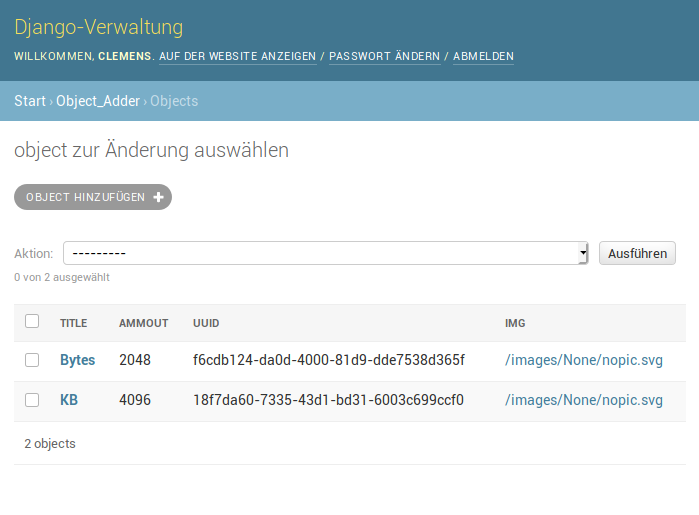
\includegraphics[width=\linewidth, height=7.5cm]{django_admin_objects.png}
\quad
\\[\baselineskip]% adds vertical line spacing
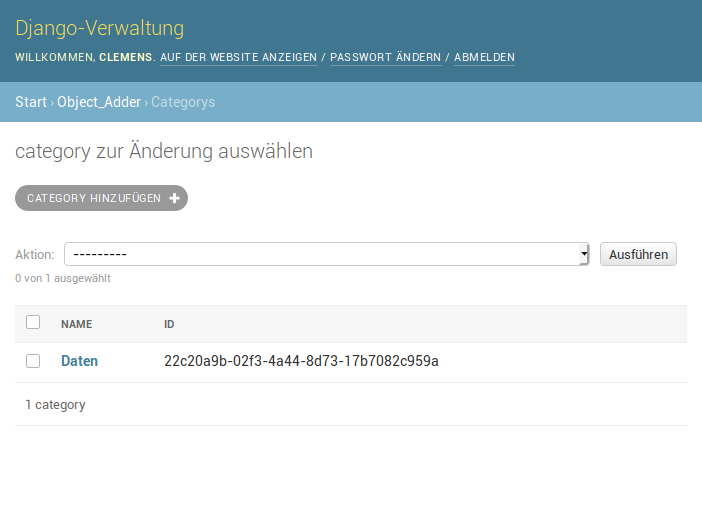
\includegraphics[width=\linewidth]{django_admin_cats.png}
\end{center}

Ohne die ''list\_display'' Angebe würde nur der primary key des Models angezeigt und das Interface sähe folgendermaßen aus:
\newline
\begin{center}
	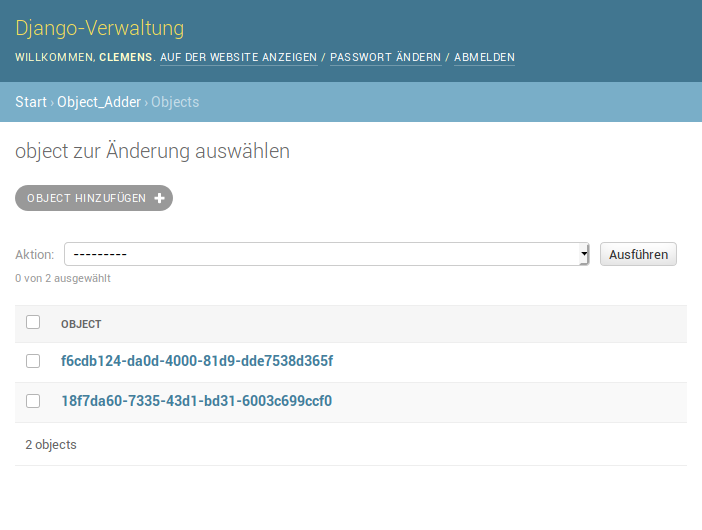
\includegraphics[width=\linewidth]{django_admin_obj_pk.png}
\end{center}
\subsubsection{apps.py}
Hier ist der Name der app definiert. Diese Datei ist außerdem notwendig, damit die App von Django als solche erkannt wird.
\begin{minted}[linenos, frame=lines, framesep=2mm]{Python}
from django.apps import AppConfig

class ObjectAdderConfig(AppConfig):
	name = 'objectadder'
\end{minted}
\subsubsection{forms.py}
In dieser Datei werden Formulare definiert. So beispielsweise das Formular zur Erstellung von Objekten und Kategorien. 


\end{document}
